\chapter{Experiments}\label{experiments}

The purpose of the application is to speed up the computation process,
thus it should be verified, whether the improvement makes sense or do
not. The improvement should correspond to the number of nodes involved
in the computation. What we wish is, that the dependence is of some
linear form, that is, the computation gets faster with every additional
node and it improves by the same steps. In this hypothetical ideal case
two nodes means two times faster computation and one hundred nodes means
one hundred times faster achievement of the result. However, this is
impossible for several reasons. At first, we must consider time that is
taken by the division process. More time is needed for transfers and
final join operation. Another problem raises because of the fact that
the transfers are quite demanding themselves so when more transfers are
ongoing at a particular moment, the initiator is more utilized and the
process could be slowed down due to this fact. This also implies that
the improvement does not raise constantly when adding more nodes.
Finally, we must consider that in the real situation delays can appear
due to technical reasons, network congestion or node failures.

\section{Approach to testing}\label{approach-to-testing}

If we want to obtain reasonable data, the measurements must be repeated
several times to prevent deviations. Also we want to keep the
measurements independent so its statistical processing is easier. Our
approach to running the tests and gathering results is described in this
chapter. Our main goal is to measure the improvement, but we would also
like to measure the impact the particular setting has on the result.

The tests were run in the school laboratory. The network consists of
several computers connected together with common ethernet twisted pair
cables. Each computer has currently installed 64 bit Gentoo
Linux\footnote{https://www.gentoo.org/} with the Linux kernel version
3.18. The machines are equipped with Intel Core i7 processors and 6 GB
of operation memory. The MTU is set to 1500B and the network uses
Gigabit Ethernet.

Because of the number of tests, it is desirable that the testing process
is automated. Because of that, special Bash script was used to run the
tests. The script is tailored to be used at the testing laboratory, so
it may need little modifications to work in some different environment.
It is distributed with the source code of the framework. To allow
automated and robust execution of the test, special functionality was
added to the program. It is invokable by option given at the start time
and causes the program to run in non-interactive mode, i.e.~keyboard
input is not accepted, the program just processes given file and ends.
This options assumes all the essential data are given when the program
is started. To keep the measurements independent, all the instances (on
every node) of the program are started at the test beginning and they
are killed in the end. Communication with the remote nodes is handled by
the ssh program. The testing script uses a special file which describes
the particular run. Working example of such file together with
explanations of the values is given below.

\begin{samepage}
\begin{verbatim}
v6 // use IPv6
/afs/ms/u/h/hudecekv/futu.avi // location of the file to be re-encoded
2 // run the whole scenario twice
slower // quality of the encoding
10000 // chunk size [KByte]
2048576 // transfer buffer size
spawn u-pl1 2221 // spawn the program on the machine 'u-pl1', use port 2221
spawn u-pl2 2222
spawn u-pl4 2224
spawn u-pl5 2225
spawn u-pl6 2226
spawn u-pl7 2227
wait 10 // wait for ten seconds before next action
kill u-pl4 // kill the instance of program running on machine 'u-pl4'
spawn u-pl8 2228
spawn u-pl9 2229
spawn u-pl10 2230
\end{verbatim}
\end{samepage}

Thanks to this mechanism, various scenarios can be run easily without
the need of human interaction.

The test data were collected by running the test ten times for the given
count of nodes. The count varied from one to ten nodes involved. Each
test was run once with chunks of 40 000 kB in size and once with 10 000
kB chunks. The same file was used each time as well as the encoding
quality. Each test gathered various results, among others the average
times needed for transfer and encoding, number of chunks, quality and
count of involved nodes. Because we had not the chance to run the tests
in some dedicated network, the computation times may vary for the given
setting depending on the current conditions. The tests showed however,
that if we multiply the average time needed to encode one chunk by the
count of chunks, the product corresponds to the time that would be taken
by the normal encoding process. This allows us to deal with the problem,
because we can compare the time with this computed estimation and the
error will be minimal. The desired values have been gathered in two
ways. Some of them, for example average transfer and encoding times, are
measured directly in the program and then outputted in special file. The
script just reads it from this file. The rest of the values is obtained
in the script.

\section{Results}\label{results}

\subsection{Linear Model}\label{linear-model}

Measurings showed, that the dependence between the number of involved
nodes and the improvement is approximately logarithmic. Work with the
data and the model was performed in the R Studio program. To evaluate
the data, simple linear regression model was used. Specifically,
subsequent formula was used:

\begin{center}
$\frac{distributed\_time}{single\_node\_time} = \beta_0 + \beta_1 \times log(neighbor\_count - 0.9)$
\end{center}

The absolute value has been added since the model fits better this way -
in the case when one neighbor is used, the distributed computation is
actually slower. The analysis of the model showed, that it makes sense
to use this model. The assumptions such as homoscedasticity (constant
variance) and independence of errors were verified using plots and
results given by the R Studio\footnote{https://www.rstudio.com/}. Some
of the mentioned outputs are given in the figures 3.1 and 3.2. We can
see, that according to the p-values corresponding to coefficients, both
of them are significant for the model. Residual standard error shows,
that the variance is not too big. In the plots we can see that residuals
has approximately constant variance. However, the second plot suggests,
that they may not be distributed normally.

\begin{figure}[h]
\begin{center}
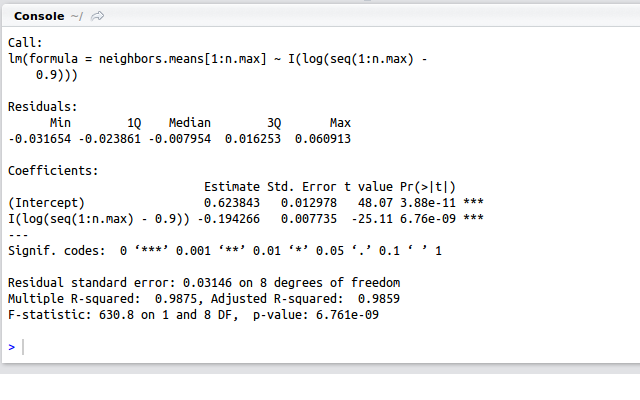
\includegraphics[scale=0.65]{./img/model.png}
\caption{Summary of the model}
\end{center}
\end{figure}

\begin{figure}[h]
\begin{center}
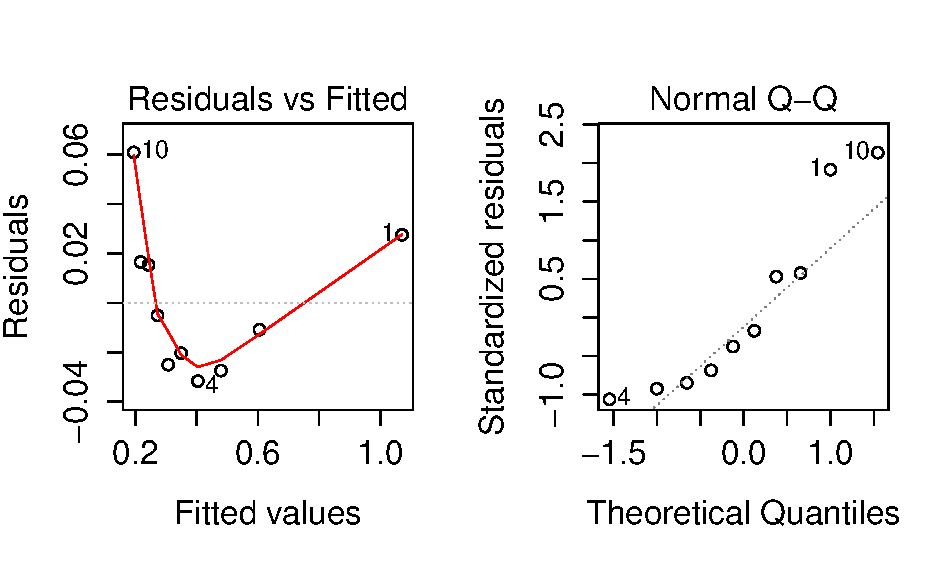
\includegraphics[scale=0.85]{./img/modelplot.pdf}
\caption{Graphical representation of the model data}
\end{center}
\end{figure}

In the figures 3.3 - 3.5 are showed the achieved results. The blue
dashed line represents the estimate which is based on the model. The
obtained data are visualized as black crosses, red squares show
respective mean values.

\begin{figure}[h]
\begin{center}
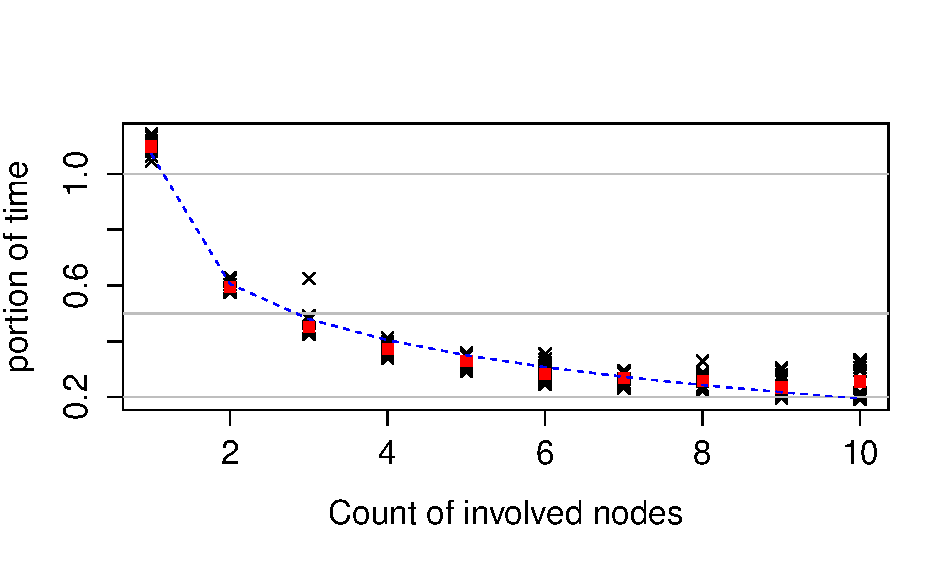
\includegraphics[scale=0.90]{./img/Rplot.pdf}
\caption{Achieved improvement - all measurements}
\end{center}
\end{figure}

\begin{figure}[h]
\begin{center}
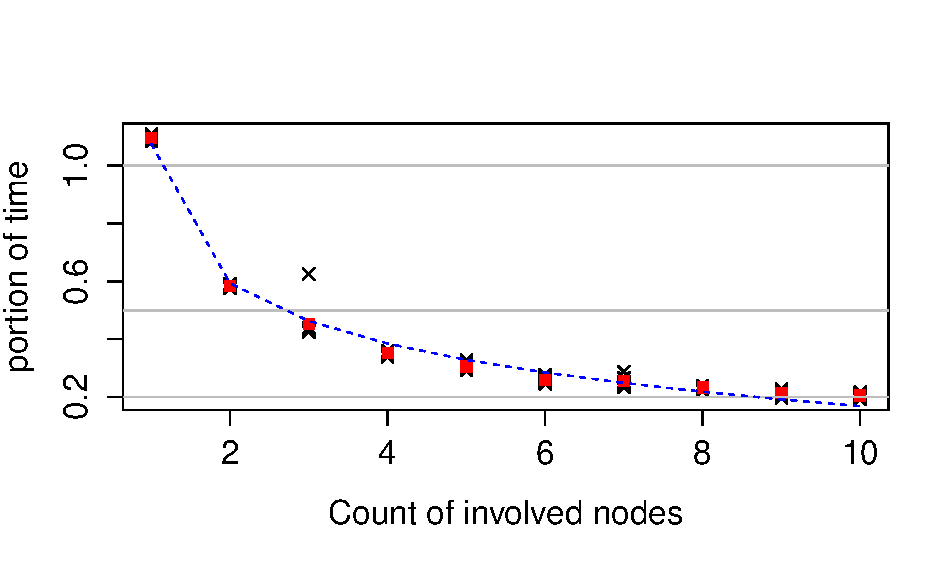
\includegraphics[scale=0.90]{./img/Rplot10k.pdf}
\caption{Achieved improvement - 10 MB chunks}
\end{center}
\end{figure}

\begin{figure}[h]
\begin{center}
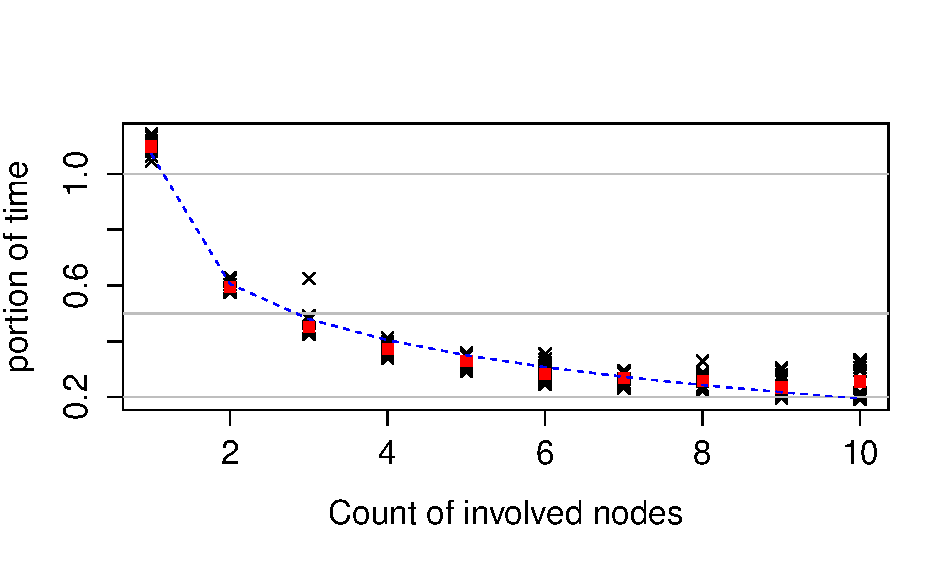
\includegraphics[scale=0.90]{./img/Rplot.pdf}
\caption{Achieved improvement - 40 MB chunks}
\end{center}
\end{figure}

In the figures 3.6, 3.7 and 3.8 are displayed ratios between particular
chunk operations. The first two shows average values per one chunk (so
the join and split times are just for an illustration), sorted in
ascending order by the chunk size, the latter shows the summations. We
can see that portion of time spent with network transfers is relatively
small in our case. These diagrams were generated using the LibreOffice
package\footnote{http://www.libreoffice.org/}

\begin{figure}[h]
\begin{center}
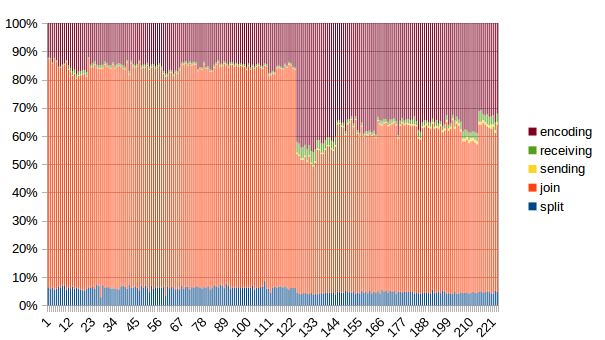
\includegraphics[scale=0.90]{./img/chunks1.png}
\caption{Comparison of operations}
\end{center}
\end{figure}

\begin{figure}[h]
\begin{center}
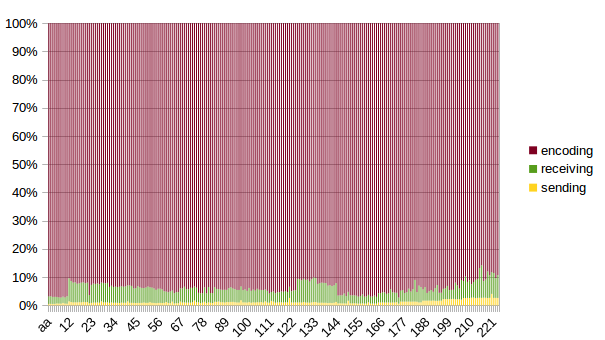
\includegraphics[scale=0.90]{./img/chunks1_2.png}
\caption{Comparison of operations}
\end{center}
\end{figure}

\begin{figure}[h]
\begin{center}
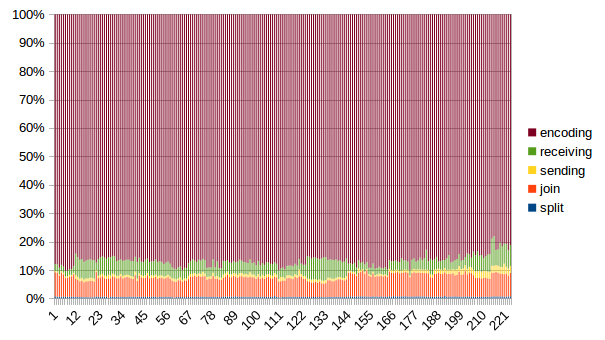
\includegraphics[scale=0.90]{./img/chunks2.png}
\caption{Comparison of operations - times summed}
\end{center}
\end{figure}

Figure 3.9. shows results of the experiment, in which one of the nodes
was killed during the process and then spawned again. As a result,
several chunks were send more times, depending on the conditions in the
network. The plot shows average number of chunk send and achieved
improvement. We can see, that resending of chunks has great impact on
the result. It introduces a thought, that sending each chunk two times
preventively could be desirable in the environments with high
probability of faults. Also, this problem could be reduced by using
smaller chunks.

\begin{figure}[h]
\begin{center}
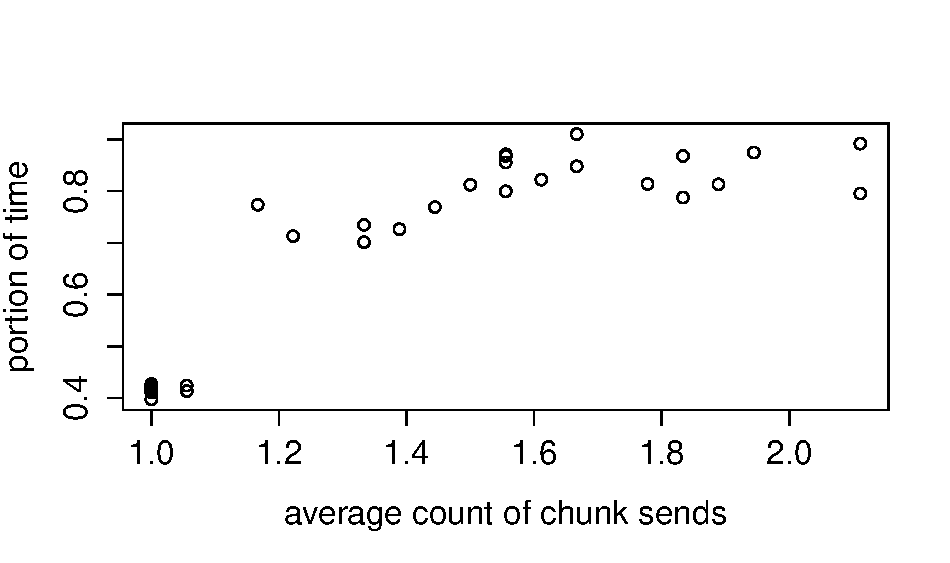
\includegraphics[scale=0.90]{./img/failures.pdf}
\caption{Impact of resending to the result}
\end{center}
\end{figure}
